% Copyright 2026 Sreeram Anil
% SPDX-License-Identifier: CC-BY-4.0
\chapter{Regularised particle filter (PF-Regularized)}
\label{ch:pfregularized}

\section*{At a glance}
\begin{tabular}{@{}l>{\raggedright\arraybackslash}p{0.76\textwidth}@{}}
Family & Sequential Monte Carlo (particle / ensemble / Gaussian sum) \\
Header & \texttt{include/estkit/particle/pf\_regularized.hpp} \\
Registered name & \texttt{PF-Regularized} ($N=500$ particles) \\
State dimension & $n_x = 4$ (cell model) — generic in $n_x, n_u, n_y$ \\
Cost per step & \SI{81.9}{\micro\second}/step ($172\times$ EKF; one extra Cholesky per resampling) \\
Memory & \SI{46.5}{\kilo\byte} \\
Primary references & \cite{musso2001regularized,arulampalam2002,silverman1986,gordon1993} \\
\end{tabular}

\section{Motivation and aerospace/BMS relevance}
Resampling is the operation that keeps a particle filter alive and the operation that kills it.
It removes the weight degeneracy that otherwise grows without bound, and it does so by drawing
children from the \emph{discrete} measure
$\hat p(\vx_k\mid\vy_{1:k}) = \sum_i w^i \delta(\vx - \vx^i)$.  Because that measure has no
density, every child is a bit-exact copy of some parent: the number of distinct particles is
non-increasing, and after enough resampling steps the cloud has collapsed onto a handful of points
--- \emph{sample impoverishment}.  For a state with substantial process noise this does not matter,
because the next time update spreads the copies apart again; for a state that is nearly an
integrator with negligible process noise --- precisely the state of charge of a battery, whose
per-step process noise standard deviation is $10^{-5}$ against a prior of $10^{-1}$ --- it matters
completely.  The cloud freezes at whatever SOC it collapsed onto and the filter degenerates into
open-loop Coulomb counting.

Musso, Oudjane and Le~Gland \cite{musso2001regularized} remove the cause rather than the symptom:
they replace the discrete measure by a kernel density estimate and resample from \emph{that}.
Children are then drawn from a continuous distribution and are almost surely distinct, so the
support of the cloud is regenerated at every resampling step without any ad-hoc jitter.  The
regularised particle filter (RPF) is the principled version of Gordon's roughening
\cite[\S4.2]{gordon1993}: the same idea, with the kernel shape, the kernel covariance and the
bandwidth all derived rather than tuned.

For a BMS this is the difference between a filter that tracks a slowly drifting SOC for a
\SI{30}{\minute} mission and one that reports a confident but stale number after the first minute.
For an aerospace certification argument it is also easier to defend: the RPF's smoothing has a
known asymptotic effect (it vanishes as $N\to\infty$), whereas an ad-hoc jitter does not.

\section{Problem statement and assumptions}
Model, inputs and outputs are exactly those of Chapter~\ref{ch:pfbootstrap},
\eqref{eq:pfb-dyn}--\eqref{eq:pfb-meas}.  The RPF makes one additional assumption that the
bootstrap filter does not:
\begin{quote}
(A3) The posterior $p(\vx_k\mid\vy_{1:k})$ has a density with respect to Lebesgue measure on
$\real^{n_x}$, and that density is square-integrable and twice differentiable.
\end{quote}
(A3) is what makes kernel density estimation meaningful and is what the mean-integrated-square-error
bandwidth rule below optimises.  It excludes models with deterministic algebraic constraints among
the states (where the posterior lives on a lower-dimensional manifold); the cell model satisfies it
because $\mQ$ is full rank.

\section{Derivation}

\subsection{From a discrete measure to a kernel density estimate}
Let $K:\real^{n_x}\to\real_+$ be a symmetric probability density (the \emph{kernel}) with
$\int \vx K(\vx)\,d\vx = \bm 0$ and $\int \vx\vx^\T K(\vx)\, d\vx = \mI$, and let $h>0$ be a
bandwidth.  Write $K_h(\vx) = h^{-n_x} K(\vx/h)$.  The RPF replaces the empirical measure by
\begin{equation}
  \hat p(\vx_k\mid\vy_{1:k}) \;=\; \sum_{i=1}^{N} w^i\, K_{h,\mS}\!\left(\vx - \vx^i\right),
  \qquad
  K_{h,\mS}(\vx) = \frac{1}{h^{n_x}\sqrt{\det \mS}}\, K\!\left(\frac{\mS^{-1/2}\vx}{h}\right),
  \label{eq:rpf-kde}
\end{equation}
where $\mS$ is the empirical covariance of the \emph{weighted} cloud,
\begin{equation}
  \bar{\vx} = \sum_i w^i \vx^i, \qquad
  \mS = \sum_i w^i (\vx^i - \bar{\vx})(\vx^i-\bar{\vx})^\T ,
  \label{eq:rpf-S}
\end{equation}
\cite[eqs.~(12)--(14)]{musso2001regularized}.  Rescaling the kernel by $\mS$ is essential: without
it a single bandwidth would have to serve states whose natural scales differ by four orders of
magnitude (here SOC $\sim 10^{-1}$ and RC voltages $\sim 10^{-3}$), and the kernel would be
degenerate in the small directions and grotesque in the large ones.

Sampling from \eqref{eq:rpf-kde} is as cheap as sampling from the discrete measure: choose a parent
index $a(j)$ by systematic resampling exactly as in \eqref{eq:pfb-systematic}, then add a kernel
draw,
\begin{equation}
  \vx^j_{\mathrm{new}} = \vx^{a(j)} + h\, \mD\, \bm{\epsilon}^j,
  \qquad \mD\mD^\T = \mS, \qquad \bm{\epsilon}^j \sim K .
  \label{eq:rpf-draw}
\end{equation}

\subsection{The optimal bandwidth}
The bandwidth is chosen to minimise the mean integrated square error between the kernel estimate
$\hat p$ and the true density $p$,
\begin{equation}
  \mathrm{MISE}(\hat p) = \E{\int \big(\hat p(\vx) - p(\vx)\big)^2 d\vx},
  \label{eq:rpf-mise}
\end{equation}
under the working assumption that the underlying density is Gaussian.  The classical result
\cite[\S4.3, eq.~(4.14)]{silverman1986} for an $n_x$-dimensional Gaussian target with a Gaussian
kernel is
\begin{equation}
  \boxed{\;
  h_{\mathrm{opt}} = A(n_x)\, N^{-1/(n_x+4)}, \qquad
  A(n_x) = \left(\frac{4}{n_x+2}\right)^{1/(n_x+4)} \; }
  \label{eq:rpf-hopt}
\end{equation}
(Musso et al.\ \cite[eq.~(15)]{musso2001regularized} give the same expression, and the analogous
constant for the Epanechnikov kernel, which is MISE-optimal among kernels but slightly more awkward
to sample in $n_x>1$).  Two features of \eqref{eq:rpf-hopt} matter in practice.  First, the
exponent $-1/(n_x+4)$ decays very slowly with $N$: at $n_x=4$, going from $N=100$ to $N=500$ shrinks
the bandwidth only from \num{0.537} to \num{0.437}.  Kernel smoothing is a weak function of sample
size --- the curse of dimensionality in disguise.  Second, $h_{\mathrm{opt}}$ is not small: at
$n_x=4$, $N=500$ it is $0.437$, so the kernel standard deviation is $44\,\%$ of the cloud standard
deviation in every principal direction.

\subsection{The bias this introduces}
Adding an independent draw of covariance $h^2\mS$ to a cloud of covariance $\mS$ produces a cloud of
covariance
\begin{equation}
  \mS_{\mathrm{new}} = (1 + h_{\mathrm{opt}}^2)\,\mS
  \;=\; 1.19\,\mS \quad\text{at } n_x=4,\ N=500 .
  \label{eq:rpf-inflation}
\end{equation}
The RPF is therefore \emph{biased}: it over-states the posterior spread by $19\,\%$ per
regularisation step and, because it is a recursion, the over-statement compounds unless the
measurement contracts the cloud by at least as much.  Musso et al.\ argue --- and the benchmark
below confirms --- that at small $N$ this bias is a bargain compared with impoverishment, and that
it vanishes as $N\to\infty$ since $h_{\mathrm{opt}}\to 0$.  The RPF is thus asymptotically
equivalent to the SIR filter of Chapter~\ref{ch:pfbootstrap} while behaving much better at the
sample sizes one can actually afford.

\subsection{Floor and cap, and why both are needed}
Equation \eqref{eq:rpf-inflation} is a growth factor of $1.19$ per step in \emph{every} direction,
including those the measurement cannot contract.  Chapter~\ref{ch:pfbootstrap},
Section~\ref{sec:pfb-battery} identified such a direction for the cell model: within one sample
interval the terminal voltage cannot separate a change in SOC from an equal and opposite change in
$v_1+v_2$.  Left alone, the kernel inflates the cloud along that direction without limit, and the
filter drifts.  Conversely, if one particle takes all the weight then $\mS \to \bm 0$ and the
kernel degenerates back to a point mass.  The implementation therefore samples from
\begin{equation}
  \bm{\Sigma}_{\mathrm{reg}} = \gamma^2 h_{\mathrm{opt}}^2 \mS + \diag(f_1^2,\dots,f_{n_x}^2),
  \qquad
  \gamma = \min_k \min\!\left(1, \frac{\varphi_{\max}\sqrt{(\mP_0)_{kk}}}{h_{\mathrm{opt}}\sqrt{\mS_{kk}}}\right),
  \qquad f_k = \varphi_{\min}\sqrt{(\mP_0)_{kk}},
  \label{eq:rpf-clip}
\end{equation}
with $\varphi_{\min} = 0.005$ and $\varphi_{\max} = 0.02$ as fractions of the prior standard
deviation.  The scalar $\gamma$ scales the \emph{whole} kernel, so its shape --- and therefore the
correlation structure that \eqref{eq:rpf-kde} is designed to respect --- is preserved; only its
overall size is bounded.  The diagonal floor is added afterwards and is the same regularisation
floor that the bootstrap filter uses.

\section{Algorithm}
\begin{algorithm}[H]
\caption{PF-Regularized --- one sampling period}
\begin{algorithmic}[1]
\Require particles $\{\vx_{k-1}^i\}$, log-weights $\{\ell^i_{k-1}\}$, $\vu_{k-1},\vu_k,\vy_k$
\State \textbf{Time update:} $\vx_k^i \gets \operatorname{constrain}(f(\vx_{k-1}^i,\vu_{k-1}) + \mL_Q\bm\xi^i)$, $i=1..N$
\State \textbf{Prior predictive:} $\yhat_k \gets \sum_i w^i_{k-1} h(\vx_k^i,\vu_k)$
\State \textbf{Weights:} $\ell^i_k \gets \ell^i_{k-1} + \log \N{\vy_k - h(\vx_k^i,\vu_k)}{\mR}$; normalise; $N_{\mathrm{eff}} \gets 1/\sum_i (w^i)^2$
\State \textbf{Moments:} $\bar{\vx} \gets \sum_i w^i\vx_k^i$; \; $\mS \gets \sum_i w^i(\vx_k^i - \bar{\vx})(\vx_k^i-\bar{\vx})^\T$
\If{$N_{\mathrm{eff}} < \beta N$} \Comment{regularised resampling}
  \State $\bm{\Sigma}_{\mathrm{reg}} \gets$ \eqref{eq:rpf-clip}; \quad $\mD \gets \operatorname{chol}(\bm{\Sigma}_{\mathrm{reg}})$
  \State parents $a(j)$ by systematic resampling \eqref{eq:pfb-systematic}
  \For{$j = 1$ \textbf{to} $N$}
    \State $\vx_k^j \gets \operatorname{constrain}\big(\vx_k^{a(j)} + \mD\,\bm{\epsilon}^j\big)$, \; $\bm\epsilon^j \sim \N{\bm 0}{\mI}$
    \State $w^j \gets 1/N$
  \EndFor
\EndIf
\State $\xhat_k \gets \sum_i w^i \vx^i_k$; \; $\mP_k \gets \sum_i w^i (\vx^i_k - \xhat_k)(\vx^i_k-\xhat_k)^\T$
\Ensure $\xhat_k$, $\mP_k$
\end{algorithmic}
\end{algorithm}

\noindent The only differences from Algorithm~1 of Chapter~\ref{ch:pfbootstrap} are lines 6--7:
the parents are perturbed by a \emph{correlated} draw whose covariance is derived from the cloud,
instead of by an independent per-coordinate jitter whose scale is derived from the cloud's bounding
box.

\section{Application to the battery model}
With $n_x = 4$ and $N = 500$ the bandwidth is $h_{\mathrm{opt}} = 0.437$ and the unclipped kernel
would have standard deviation $0.437\sqrt{\mS_{kk}}$ in coordinate $k$.  During the initial
transient the SOC spread is $\sqrt{\mS_{\soc\soc}}\approx 0.1$, so the kernel would put
\num{0.044} of SOC on each child --- far more than the \num{0.003} that a single voltage sample can
resolve --- and the cap \eqref{eq:rpf-clip} binds, limiting it to $0.02\times0.1 = \num{0.002}$.
Once the filter has converged, $\sqrt{\mS_{\soc\soc}}$ falls to a few $10^{-3}$, the kernel gives
$0.437\times 3\times10^{-3} \approx 1.3\times10^{-3}$ and the cap releases: the RPF then behaves
exactly as Musso et al.\ intended, with a bandwidth that tracks the posterior.  The floor takes
over only if a single particle ever takes the entire weight.

Because the kernel is drawn with the \emph{full} covariance $\mS$ rather than its diagonal, the
children inherit the SOC--$v_2$ correlation that the measurement has built up.  This is the
qualitative advantage over the diagonal roughening of Chapter~\ref{ch:pfbootstrap}: the perturbation
is applied along the cloud's own principal axes, so it explores the directions the data have left
undetermined instead of pushing equally hard along all four coordinates.  The measured effect is
visible in the scenarios where the posterior is genuinely anisotropic --- \code{combined}
(\SI{2.51}{\percent} against \SI{2.76}{\percent} for the bootstrap filter) and \code{preisach}
(\SI{1.00}{\percent} against \SI{1.08}{\percent}).  Neither margin is large, but both have the
expected sign.

\section{Implementation notes}
\emph{Cost.}  One extra $n_x\times n_x$ Cholesky and $N n_x^2$ multiply-adds per resampling step
relative to \estname{PF-Bootstrap} --- about \num{6000} flops per step at $N=500$, $n_x=4$.
Measured \SI{81.9}{\micro\second}/step against \SI{76.4}{\micro\second} for the bootstrap filter,
i.e.\ \SI{7}{\percent}, which matches that flop estimate.  In single precision the filter is if
anything slightly more accurate (\SI{0.08}{\percent} against \SI{0.09}{\percent} on \code{nominal},
Table~\ref{tab:float}): the kernel draw is dominated by the Cholesky of a well-conditioned
$4\times4$ matrix and has no dynamic-range problem.  The empirical covariance \eqref{eq:rpf-S} is not extra work, because the
filter must compute $\mP_k$ for \code{soc\_std} anyway; the implementation calls
\code{refresh\_moments()} before the resampling decision and reuses the result as $\mS$.

\emph{Memory.}  Identical to \estname{PF-Bootstrap} (\SI{46.5}{\kilo\byte}): the children are
written into the scratch buffer and copied back.  The in-place scheme of Chapter~\ref{ch:pffast}
does \emph{not} transfer directly, because in the RPF every child is modified after copying, so the
"no-copy when $n^i=1$" shortcut buys nothing; a variant that draws the kernel perturbation in place
after an in-place redistribution would recover the memory at the cost of one extra pass.

\emph{Kernel choice.}  The Gaussian kernel is used because it is trivially sampled from the
Cholesky factor already available, because it is closed under the linear rescaling by $\mS^{1/2}$,
and because the constant $A(n_x)$ in \eqref{eq:rpf-hopt} is then exact rather than asymptotic.  The
Epanechnikov kernel has a marginally smaller MISE constant but a heavier sampler and compact
support, which can leave a child outside the feasible set of a constrained model.

\emph{Guards.}  $\bm{\Sigma}_{\mathrm{reg}}$ is factorised with \code{cholesky\_safe}, which adds
diagonal jitter if the empirical covariance is numerically indefinite (it can be, when all weight
sits on one particle).  Children are projected with \code{constrain()}, so SOC stays in
$[-0.05, 1.05]$ and the hysteresis state in $[-1,1]$ regardless of the kernel draw.

\section{Benchmark results}
% Copyright 2026 Sreeram Anil
% SPDX-License-Identifier: CC-BY-4.0
\begin{table}[H]\centering\footnotesize\setlength{\tabcolsep}{4pt}
\caption{PF-Regularized: cell-level benchmark on the eVTOL mission (mean over seeds; RMSE and max error in \% SOC; $t_\mathrm{conv}$: first time the error stays below 2\,\% for 60\,s, -- = never; EKF reference: steady-state RMSE of the plain EKF on the same data).}\label{tab:cell_PFRegularized}
\begin{tabular}{llrrrrrcrr}\toprule
plant & scenario & RMSE & RMSE$_\mathrm{ss}$ & max & $t_\mathrm{conv}$ [s] & RMSE$_v$ [mV] & div. & EKF ref. & ns/step \\ \midrule
ECM & nominal & 0.16 & 0.12 & 0.80 & 0 & 0.83 & no & 0.05 & 81850 \\
ECM & init\_error & 0.46 & 0.11 & 5.01 & 9 & 2.21 & no & 0.05 & 81720 \\
ECM & current\_bias & 0.96 & 0.90 & 2.54 & 0 & 0.87 & no & 0.61 & 81893 \\
ECM & noise\_step & 0.42 & 0.50 & 1.78 & 0 & 2.94 & no & 0.12 & 95646 \\
ECM & outliers & 0.47 & 0.34 & 1.88 & 0 & 1.56 & no & 0.21 & 84234 \\
ECM & cold & 0.30 & 0.24 & 1.17 & 0 & 1.92 & no & 0.16 & 81836 \\
ECM & hot & 0.12 & 0.06 & 0.77 & 0 & 0.60 & no & 0.03 & 81818 \\
ECM & aged\_cell & 3.15 & 2.51 & 13.41 & 0 & 5.03 & no & 1.52 & 85141 \\
ECM & param\_mismatch & 2.07 & 1.88 & 8.83 & 0 & 3.37 & no & 1.36 & 84044 \\
ECM & sensor\_dropout & 0.39 & 0.12 & 4.60 & 0 & 1.43 & no & 0.46 & 81753 \\
ECM & preisach & 1.39 & 1.00 & 4.28 & 217 & 0.87 & no & 0.20 & 82116 \\
ECM & combined & 3.08 & 2.51 & 15.29 & 180 & 6.47 & no & 12.44 & 85666 \\
\midrule
SPM & nominal & 0.89 & 0.64 & 3.25 & 0 & 1.08 & no & 3.73 & 79446 \\
SPM & init\_error & 1.60 & 0.71 & 5.01 & 319 & 2.21 & no & 3.81 & 79652 \\
SPM & current\_bias & 0.86 & 0.67 & 4.32 & 0 & 1.15 & no & 5.69 & 79534 \\
SPM & noise\_step & 1.20 & 1.15 & 3.27 & 0 & 3.08 & no & 3.30 & 92918 \\
SPM & outliers & 1.12 & 0.81 & 4.71 & 0 & 1.76 & no & 1.99 & 81587 \\
SPM & cold & 3.67 & 3.91 & 13.33 & 369 & 7.08 & no & 7.35 & 81377 \\
SPM & hot & 0.63 & 0.54 & 2.31 & 0 & 0.74 & no & 2.16 & 79680 \\
SPM & param\_mismatch & 2.12 & 1.35 & 7.23 & 0 & 2.24 & no & 3.13 & 80640 \\
SPM & sensor\_dropout & 1.02 & 0.70 & 6.89 & 0 & 2.04 & no & 5.31 & 79813 \\
\bottomrule\end{tabular}\end{table}

\begin{figure}[H]\centering
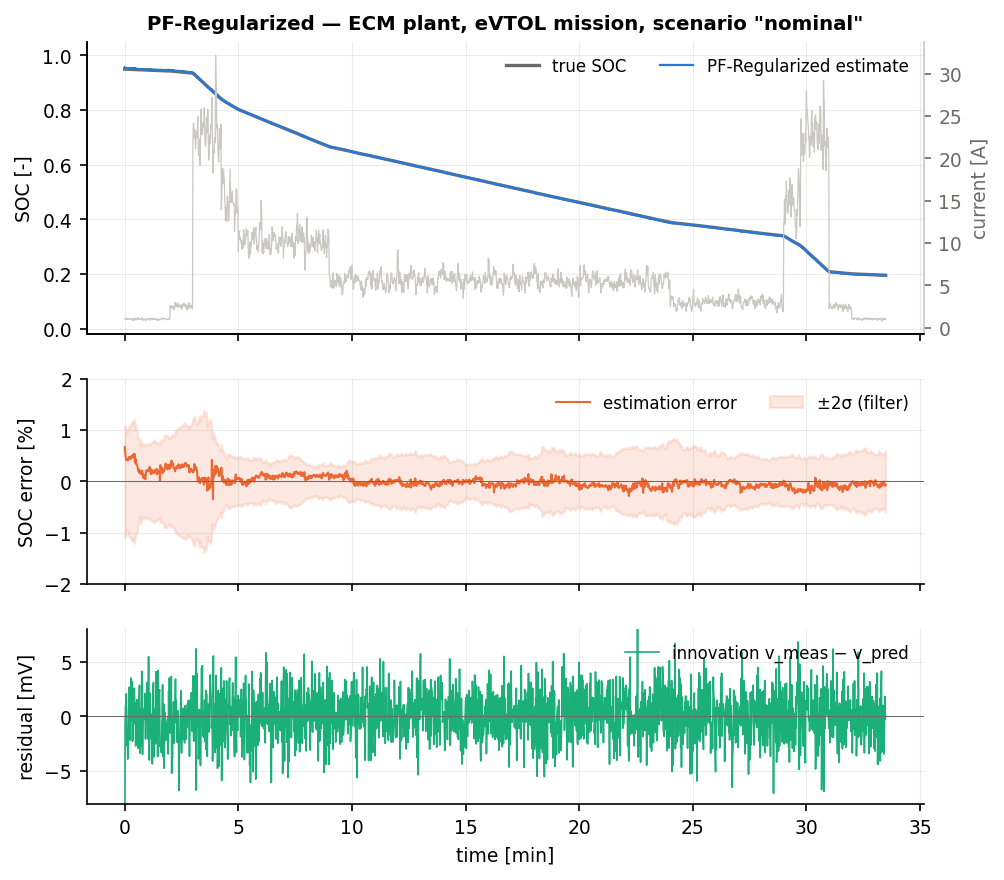
\includegraphics[width=\textwidth]{figures/cell_PFRegularized_nominal.png}
\caption{PF-Regularized on the nominal eVTOL mission: true and estimated SOC (top), estimation
error with the $\pm2\sigma$ band (middle), voltage residual (bottom).}
\end{figure}
\begin{figure}[H]\centering
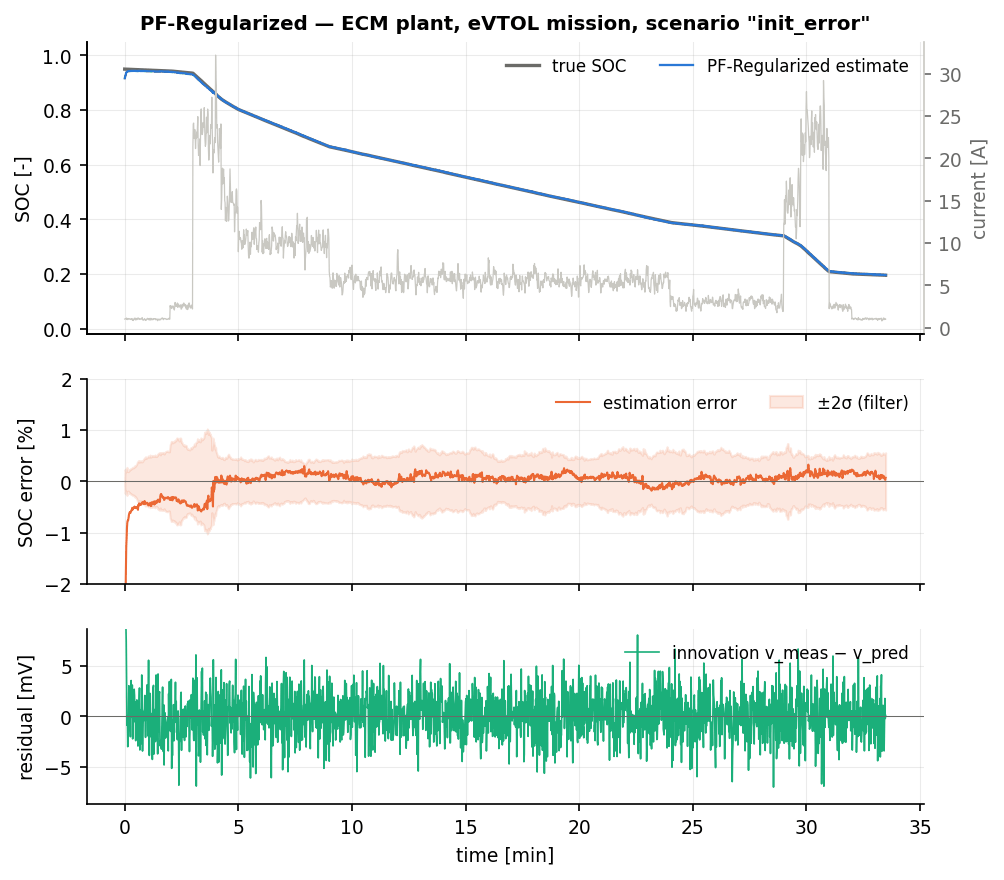
\includegraphics[width=\textwidth]{figures/cell_PFRegularized_init_error.png}
\caption{PF-Regularized with a \SI{35}{\percent} initial SOC error: the kernel is capped during the
transient and releases to the MISE-optimal bandwidth once the cloud has converged.  This is the
fastest recovery of the four full-state particle filters (\SI{9}{\second}).}
\end{figure}
\begin{figure}[H]\centering
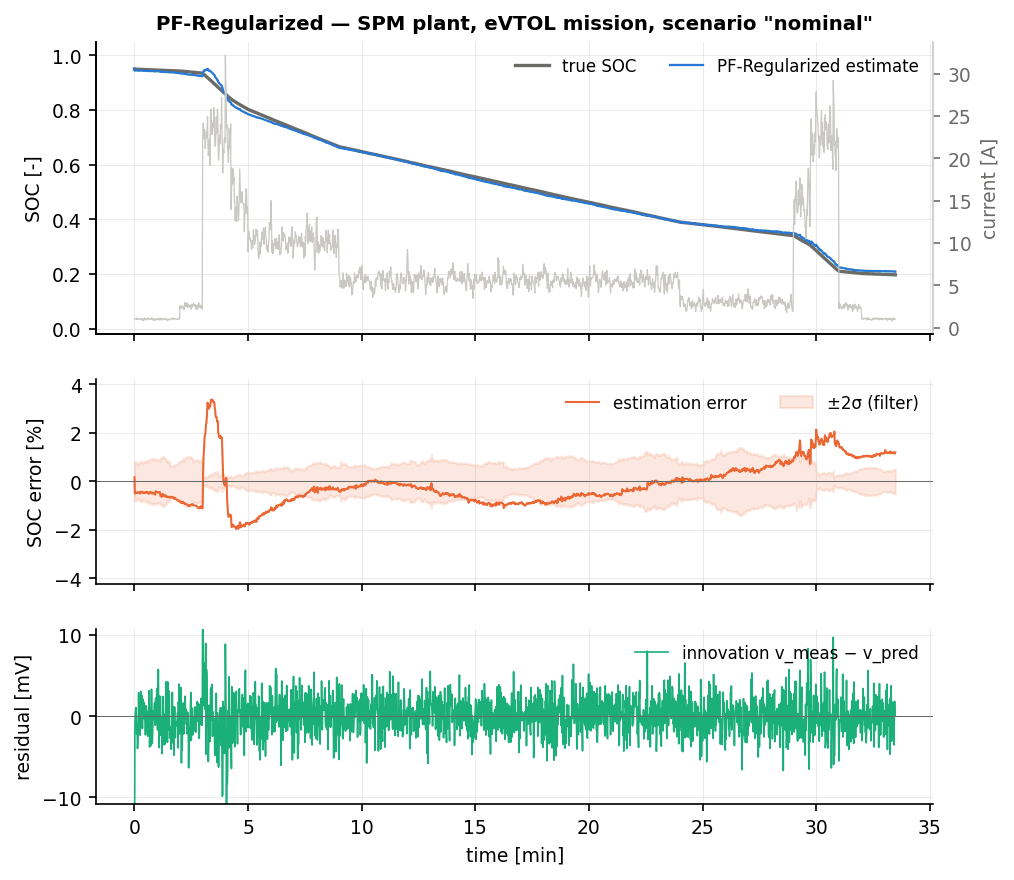
\includegraphics[width=\textwidth]{figures/cellspm_PFRegularized_nominal.png}
\caption{PF-Regularized on the electrochemical (SPM) plant, nominal mission.}
\end{figure}

\paragraph{ECM plant.}  On \code{nominal} the RPF reaches $\mathrm{RMSE} = \SI{0.16}{\percent}$,
$\mathrm{RMSE}_{\mathrm{ss}} = \SI{0.12}{\percent}$, maximum error \SI{0.80}{\percent}, immediate
convergence and a voltage residual of \SI{0.83}{\milli\volt}.  It is the most accurate of the four
full-state particle filters on this scenario (bootstrap \SI{0.16}{\percent}, auxiliary
\SI{0.15}{\percent}, fast \SI{0.18}{\percent}), though still a factor \num{2.4} behind the EKF's
\SI{0.05}{\percent} on a plant whose model is exact.  With a \SI{35}{\percent} initial error it
converges in \SI{9}{\second} --- by a wide margin the fastest of the four (bootstrap
\SI{73}{\second}, fast \SI{5}{\second} but with twice the peak error, auxiliary
\SI{155}{\second}) --- to $\mathrm{RMSE}_{\mathrm{ss}} = \SI{0.11}{\percent}$, the best value of
the four.  The advantage is small but systematic and lands exactly where the theory predicts: the
correlated kernel beats diagonal jitter when the posterior is anisotropic, which is the case during
and after a large transient.

Elsewhere on the ECM plant it is the most consistent member of the family: \code{cold}
\SI{0.24}{\percent} and \code{hot} \SI{0.06}{\percent} (both the best of the four, and \code{hot}
matches the UKF), \code{sensor\_dropout} \SI{0.12}{\percent} against \SI{0.46}{\percent} for the
EKF, \code{outliers} \SI{0.34}{\percent}, \code{noise\_step} \SI{0.50}{\percent},
\code{current\_bias} \SI{0.90}{\percent}, \code{combined} \SI{2.51}{\percent} against
\SI{12.44}{\percent} for the EKF.  It shares the family's two weaknesses --- \code{aged\_cell}
\SI{2.51}{\percent} and \code{param\_mismatch} \SI{1.88}{\percent} (the worst of the four, against
\SI{1.36}{\percent} for the EKF), because no amount of sampling fidelity compensates a model whose
capacity is \SI{15}{\percent} wrong --- and it loses, like every particle filter here, on
\code{preisach} (\SI{1.00}{\percent} against \SI{0.20}{\percent} for the EKF) now that the
corrected hysteresis sign makes the unmodelled Preisach loop act as a slow voltage bias rather than
as extra spread.

\paragraph{SPM plant.}  Against the electrochemical plant the RPF is one of the two best methods in
the whole family: $\mathrm{RMSE}_{\mathrm{ss}} = \SI{0.64}{\percent}$ on \code{nominal} against
\SI{3.73}{\percent} for the EKF and \SI{3.96}{\percent} for the UKF --- a factor of \num{5.8} ---
with immediate convergence.  \code{current\_bias} is \SI{0.67}{\percent} against
\SI{5.69}{\percent}, \code{hot} \SI{0.54}{\percent} against \SI{2.16}{\percent},
\code{param\_mismatch} \SI{1.35}{\percent} against \SI{3.13}{\percent}, \code{sensor\_dropout}
\SI{0.70}{\percent} against \SI{5.31}{\percent} and \code{cold} \SI{3.91}{\percent} against
\SI{7.35}{\percent}; nothing diverges.  The kernel is the reason it edges ahead of plain roughening
here.  A structured \SI{4}{\milli\volt} residual must be absorbed somewhere, and the only
representation that keeps it out of the SOC is one in which SOC and the slow RC state are free to
move together; the regularisation kernel is drawn with the \emph{full} empirical covariance, so its
perturbations lie along the cloud's own principal axes --- precisely the $(\soc, v_2)$ ridge that
the measurement leaves undetermined within one step --- instead of pushing equally hard along all
four coordinates.  The particle cloud is therefore never forced into the linearised $(\soc,v_2)$
trade-off that a Kalman gain has to make, and the residual shows up as voltage-residual RMSE
(\SI{1.08}{\milli\volt}) rather than as SOC bias.

\section{Summary}
The regularised particle filter is the bootstrap filter with its resampling step repaired: children
are drawn from a kernel density estimate instead of from a discrete measure, so the cloud
regenerates its own support and sample impoverishment is eliminated by construction rather than by
an ad-hoc jitter.  The kernel covariance is the empirical covariance of the weighted cloud and the
bandwidth is the MISE-optimal $h_{\mathrm{opt}} = A(n_x)N^{-1/(n_x+4)}$, so the only free parameter
is the choice of kernel.  It costs \SI{7}{\percent} more than \estname{PF-Bootstrap} and returns the
best nominal accuracy and the fastest initial-error recovery of the full-state particle filters on
the ECM plant (\SI{0.12}{\percent}, \SI{9}{\second}) and \SI{0.64}{\percent} against the EKF's
\SI{3.73}{\percent} on the electrochemical plant.  Use it in place of the bootstrap filter whenever
the process noise is small compared with the measurement information --- which, for state of
charge, is always.  Do not expect it to rescue a mis-parameterised \emph{capacity}
(\code{aged\_cell}, \code{param\_mismatch}): that is the job of Chapter~\ref{ch:rbpf}, which samples
fewer states, or of joint state/parameter estimation.
